Reinforcement Learning (RL) is an area of machine learning, closely tied to behavioral psychology, concerned with how agents should behave in their environment as to maximize some notion of utility function. Being inspired from psychology, we can say that this area is the closer to how humans and other beings learn.  The agent has to explore  environment, collecting data on its interactions and using them to make informed decisions in the future. In a way this process is similar to a baby exploring his surroundings and playing in a playground. The process is formalized in Figure \ref{fig:rl_framework}.\par
\begin{figure}
  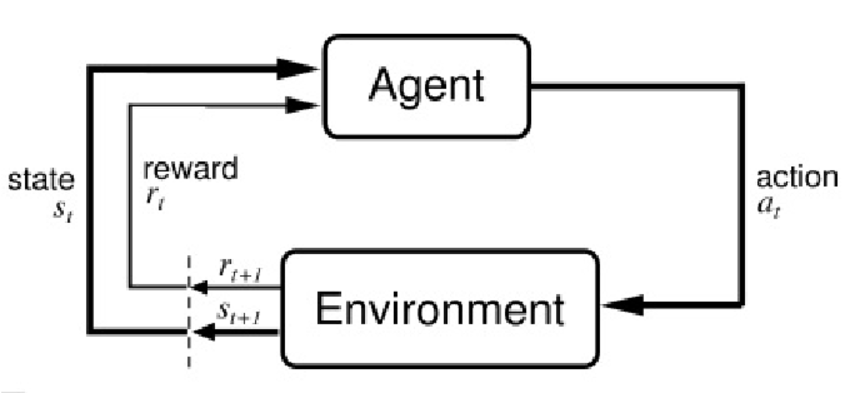
\includegraphics[width=\linewidth]{RL.png}
  \caption{The Reinforcement Learning framework ~\cite{Sutton:1998:IRL:551283}}
  \label{fig:rl_framework}
\end{figure}
The main driver of the agent's behavior is the reward signal it receives from the environment.  In the baby's case, the activity of exploring the playground and playing, is driven by an intrinsic motivation of human beings to explore our surroundings and understand them better, which in this case can be seen as an internal, or intrinsic reward signal. Other examples include teaching rats how to solve a maze by giving them food if they reach the end. In this case the reward signal is external or extrinsic. In either case the reward function  specifies the task the agent has to learn. We assume that the reward is given to the agent after every action but in the most interesting and complicated cases actions might affect not only the immediate rewards but also future rewards. So the agent must have the ability to map the sensations it gets from the environment (states) to actions, keeping in mind the effects of these actions in the future. This kind of problems are best described in the Markov Decision Process (MDP) framework.\par
Reinforcement Learning is fundamentally different from supervised learning. In the latter, learning is conducted on a training set of labeled samples provided by an external knowledgeable source (supervised)~\cite{hastie_09_elements-of.statistical-learning}. Each sample is a representation of the situation together with specification of the correct behavior of the system in this situation. This kind of learning is used to generalize from this training dataset, and apply a correct behavior in future situations not present in the train set. Even though it is a really important part of machine learning, supervised learning alone is not enough to deal with control problems. In interactive problems it is often impractical to collect these datasets of the desired behavior, and even if this data is available it might be unreliable so the agents must be able to learn from their own experience. \par
Nonetheless supervised learning is often used together with reinforcement learning to tackle control problems. A famous example is the original AlphaGo~\cite{Silver_2016}, the first computer program able to beat an expert player in the ancient Chinese game of Go. The program was first trained to mimic the moves of expert players by using a database of historical moves containing more than 30 million moves. After it reached a certain level of mastery, using reinforcement learning methods,  the program was trained from experience by playing against other instances of itself. Even though this was a milestone in Artificial Intelligence, it was surpassed by the latest version of the program, Alpha Go Zero~\cite{silver2017mastering} , which skipped the initial supervised learning and learned to play the game totally by scratch and was able to beat the original game, 100 times in 100 games, showing the importance of reinforcement learning in control problems.\par
Reinforcement learning is also different from unsupervised learning which in literature is typically refereed as the area of machine learning concerned with finding structure hidden in large sets of unlabeled data~\cite{hastie_09_elements-of.statistical-learning}. Even though both rely on learning from unlabeled data, reinforcement learning is concerned with maximizing a reward signal received from the environment rather than discovering hidden features of the environment. Discovering features of the environment might be useful to reach the goal, but alone it is not enough to maximize the reward. For this reason, reinforcement learning is considered as a third machine learning paradigm~\cite{Sutton:1998:IRL:551283}.\par
Another aspect that distinguishes reinforcement learning form other paradigms of machine learning is the exploration vs exploitation dilemma, which is one of the greatest (if not the greatest) challenges of reinforcement learning and it does not arise in the other machine learning paradigms. Agents must be able  to apply the “best” actions in each situation  they face. To evaluate the value of each action they use the knowledge acquired from the interaction with the environment and to discover the best actions they need to explore the environment by applying new actions. So neither exploration or exploitation can be used exclusively to reach the goal of maximizing the reward. How do you balance the two? This dilemma is even more important in stochastic tasks, where actions have to be tried multiple times before having a reliable estimate of their value. This problem has been studied extensively for decades but no definitive solution has been found so far.\par
In this thesis, to address the exploration vs exploitation dilemma, we will turn to a distributional approach to Reinforcement Learning. The common approach to reinforcement learning models the expected cumulative reward received from each action in given states. By explicitly modeling the distribution of the return estimate, instead of the expected value we are able to have a better estimate of the value of each action and to quantify the exploration dilemma, thus making better decisions.~\cite{Dearden98bayesianq-learning}\par
This chapter is meant to introduce main concepts of reinforcement learning used in further chapters. The chapter is organized as follows. We start in Section ~\ref{MDPs} where we introduce the concept of Markov decision process, the notion of value function and we formalize the optimality criteria. Section ~\ref{planning_mdps} briefly presents the notion of planning in MDPs and  dynamic programming, the standard approach to solve MDPs, when the model of the environment is available. Section ~\ref{reinforcement_learning} gives a classification of RL algorithms and describes the most important model-free algorithms. In Section ~\ref{sec:function_approximation} we shortly discuss function approximation. Finally, Section ~\ref{distributional_rl_section} is devoted to distributional RL and the fundamental importance of the value distribution.
\section{Markov Decision Processes} \label{MDPs}
Markov Decision Processes (MDPs) provide a mathematical framework for modeling sequential  decision making problems in situations where the outcomes are partly random and partly in control of a goal-directed agent, which interacts with an environment by performing actions and sensing perceptions. In this thesis we consider discrete time  MDPs, in which the agent has to decide which action to take in each state so that he maximizes his utility function. At each time step the agent perceives a state  from the environment, and after choosing an action he perceives the next state he moved to and a reward signal associated with this transition, called  immediate reward. Usually the utility function of the agent is some sort of cumulative reward calculated on an extended time frame. Maximizing the immediate rewards might not be enough to maximize the cumulative reward so many times the agent has to sacrifice immediate rewards to gain in the long  term.\par
Markov Decision Processes are an extension of Markov Chains. The difference is the addition of actions (allowing choice of the agent) and rewards (providing motivation to the agent). So if we have only one action , and all the rewards are the same  an MDP reduces to a Markov Chain. These processes are called Markov, because they have what is known as the Markov property, that is, that given the current state and action, the next  state is independent of all the previous states and actions. The current state captures all that is relevant about the world in order to predict what the next state will be.   
\subsection{Definitions}
Different definitions are available in literature. We consider the following one:
\begin{definition}
	A Markov Decision Process is a \emph{tuple} $\mathcal{M= (S, A, P, R, \mu, \gamma)}$ ,
where:
\end{definition}
\begin{itemize}
\item $\mathcal{S}$ is a \emph{non-empty measurable} set , called \emph{state space};
\item $\mathcal{A}$ is a \emph{non-empty measurable} set , called \emph{action space};
\item $\mathcal{P}$ is a function $\mathcal{P: S\times A\rightarrow}\Delta \mathcal{S}$ called \emph{transition model}, that for all  $s \mathcal{ \in S}$ and for all  $a\mathcal{\in A}$, assigns $\mathcal{P}(\cdot\mid s,a)$, a probability measure over $\mathcal{S}$,$P(\cdot\mid s,a)$ being the corresponding probability density function;
\item $\mathcal{R}$ is a function $\mathcal{R: S\times A \times S\rightarrow \Delta \mathbb{R}}$ called \emph{the reward function}, that for all  $s,s' \mathcal{ \in S}$ and for all  $a\mathcal{\in A}$, assigns $\mathcal{R}(\cdot\mid s,a,s')$, a probability measure over $\mathbb{R}$,R$(\cdot\mid s,a,s')$ being the corresponding probability density function and R(s,a)= $\mathbb{E}_{\substack{\text{$ s'\sim P(\cdot\mid s,a)$} \\ \text{$r \sim R(\cdot\mid s,a,s')$}}} [r] $ is the state-action expected reward;
\item $\mu$ is a probability measure over $\mathcal{S}$ called distribution of the initial states, $\mu(\cdot)$ being the probability density function;
\item $\gamma \in [0,1]$ is the \emph{discount factor}. 
\end{itemize} \par
The state space $\mathcal{S}$ and the action space $\mathcal{A}$ define the sensor and actuator possibilities of the agent. They can be either finite or infinite, discrete or continuous. Sometimes not all the actions are performable in all states, in this case it is convenient to define the set $\mathcal{A}(s)$ for all $s\mathcal{ \in S}$ which is the set of actions available in state s, therefore $\mathcal{A}= \bigcup_{s∈S}A(s)$\par
The immediate payoff is modeled by means of a scalar reward, that given the current state $s$, the current action $a$ and the next state $s′$ assigns for all Borel sets $A \in B(\mathbb{R})$ the quantity $R(A|s, a, s′)$ that is the probability to get a payoff in $A$ by starting from state $s$, performing action $a$ and ending up in state $s′$. $R(\cdot|s, a, s′)$ is the corresponding density function. In most common applications the state-action expected reward $R(s, a)$ is used,  defined as the expected value of the reward taken over all next states $s′$ and all real rewards $r$. Sometimes it is convenient to consider the state-action-state expected reward $R(s, a, s′) = \mathbb{E}_{r∼R(\cdot|s,a,s′)} [r]$. We will also assume that the immediate reward is upper bounded in absolute value, \ie $\parallel R\parallel_{\infty} = \max_{s\in \mathcal{S}} \max_{a \in \mathcal{A}} \mid R(s,a)\mid \leq M < +\infty $.\par
The reward function ultimately defines the goal of the agent in its environment. Is a scalar reward enough to specify every goal? Sutton and Burto~\cite{Sutton:1998:IRL:551283} hypothesize that all that we call \emph{goal} can be expressed as maximizing the cumulative sum of a received scalar reward signal. Although not proven, this hypothesis is so simple and powerful that we need to disprove it before looking for something more complicated.\par
The time is modeled as a discrete set of time steps, typically represented as a sequence of natural numbers $\mathcal{T} = {0, 1, \ldots, T }$ where $T$ is called \emph{horizon} and can be either finite $T \in \mathbb{N}$ or infinite $T = \infty$. In the former case the MDP is said to be \emph{finite horizon}, otherwise it is called \emph{infinite horizon}. An MDP is said episodic if the state space contains a \emph{terminal} (or absorbing) state, \ie a state $s$ from which no other states can be reached (for all actions $a \in \mathcal{A}, P(s|s,a)= 1$). Typically, it is assumed that all actions performed in a terminal state yield zero reward.\par
The discount factor $\gamma$, which is typically strictly less than 1, causes rewards perceived further in time to be weighted less. This is especially important in infinite horizon MDPs, but might be useful also in finite horizon cases. A typical example where applying a discount factor less than 1 are financial applications where receiving monetary rewards in the present usually is more valuable than receiving them in the future due to the interest rate.\par
To recap, the dynamics of MDPs are as follows. We start from an initial state $s_{0}$ drawn from the initial state distribution $\mu$. At each time step the agent choses an action from the available set of actions $A(s)$. Following the transition model $P(\cdot \mid s,a)$ it ends in state $s'$ and it observes the reward signal $r$ drawn from the reward model $R(\cdot \mid s,a,s')$. By repeatedly applying these activity the agent traverses a sequence of states collecting a sequence of rewards. Maximizing the ($\gamma$ discounted) cumulative sum of these rewards is the agents goal.
\subsection{Policies}
As we said before the goal of an agent is to maximize some sort of cumulative reward by taking actions that produce larger rewards. Generally the agent uses the history of states he has traversed ($s_0, s_1...$) to make decision on future actions as to maximize his utility function. The set of rules mapping the agents history to actions are called \emph{policies}. But because MDPs have the Markovian property, the current state ,$s_t$ is enough to determine the next action $a_t$~\cite{Sutton:1998:IRL:551283}. These kind of policies are called, not surprisingly, Markovian Policies. Moreover if the actions mapped are not dependent on the time step $t$, the policy is called stationary. In this thesis,for simplicity, when we use the term policy we will refer to Markovian Stationary Policies. More formally:
\begin{definition}
	A Markovian Stationary Policy $\pi$ is a function $\pi:\mathcal{S}\rightarrow \Delta(A)$ that for every state $s \in \mathcal{S}$ maps a probability distribution, $\pi(\cdot \mid s)$, over the action space $\mathcal{A}$. If the policy is deterministic then $\pi:\mathcal{S}\rightarrow A$
\end{definition}
The goal of reinforcement learning becomes finding the policy that maximizes the cumulative reward collected.
An MDP paired with a policy $\pi$ induces what in literature is called a \emph{Markov Reward Process} denoted by the tuple $\mathcal{(S,P^\pi,R^\pi,\gamma,\mu)}$. For all states $s \in \mathcal{S}$, $\mathcal{P^\pi}(\cdot \mid s)$ is a probability measure over $\mathcal{S}$. $P^\pi$ is the probability density function obtained by marginalizing the transition model of the MDP, $\mathcal{P}$ over the actions:
\begin{equation}
	P^\pi(s'|s)=\sum_{a \in \mathcal{A}} \pi(a|s)P(s'|s,a) \qquad \forall s,s' \in \mathcal{S}
\end{equation}
$P^\pi(s'|s)$ gives the probability of ending up in state s', starting from state s, in one time step. Similarly,$\mathcal{R^\pi}(\cdot|s,s′)$ for all $s,s′\in \mathcal{S}$ is a probability measure over $\mathbb{R}$ with the corresponding density function $R$ obtained from the reward model of the MDP as:
\begin{equation}
	R^\pi(r|s,s')=\sum_{a \in \mathcal{A}} \pi(a|s)\mathcal{R}(r|s,s',a) \qquad \forall s,s' \in \mathcal{S}
\end{equation}
MRPs are a suitable model for uncontrolled processes. The notion of action disappears and they can be used to model stochastic processes taking place in the environment and producing rewards. By further removing the concept of reward from the MRPs, as mentioned before we are left with Markov Chains or Markov Processes.
\subsection{Utility Functions and Value Functions}
Given a policy $\pi$, played by an agent in an MDP, it is possible to define the utility of each state. While the reward signal measures the immediate payoff the agent experiences, the utility function of a state measures the reward in a long run. The utility function is calculated over trajectories, and measures how ``good'' that trajectory is to the agents. Typically the utility is a sum (possibly discounted) of the rewards collected during the trajectory , even though there are other types of utility functions defined in literature~\cite{Puterman:1994:MDP:528623}. \par
If $\tau$ is a trajectory the agent followed under policy $\pi$,starting form the initial state distribution $\mu$, the expected discounted sum of rewards is defined as:
\begin{equation}
		J^{\pi}=E_{\tau \sim p(\cdot |\mu,\pi,\mathcal{P})}\left[ \sum_{t=0}^{T(\tau)} R(s_{\tau,t},a_{\tau,t})\right]
\end{equation}
where :
\begin{itemize}
\item $T(\tau)$ is the length of trajectory $\tau$;
\item $s_{\tau,t}$ is the state where the agent is in the t-th time step of trajectory $\tau$;
\item $a_{\tau,t}$ is the action taken in the t-th time step of trajectory $\tau$.
\end{itemize}
To avoid the potential divergence of the utility function in the case of infinite MDP, a discount factor is introduced and the utility function becomes the discounted expected cumulative reward also known as \emph{expected return}~\cite{Sutton:1998:IRL:551283}.
\begin{equation}
		J^{\pi}=E_{\tau ~p(\cdot |\mu,\pi,\mathcal{P})}\left[ \sum_{t=0}^{T(\tau)} \gamma^{t}(s_{\tau,t},a_{\tau,t})\right].
\end{equation}
By introducing the discount factor we avoid the divergence of this measure, holding the assumption that the reward signal is upper bounded. The discount factor is open to multiple interpretations. From an economical/financial point of view the discount factor accounts for the fact that an agent might be more interested in a payoff obtained in the near future rather than a payoff obtained far in the future. Values of $\gamma$ close to 0 lead to a "miopic” evolution (at the limit in which $\gamma$ = 0 the agent is interested only in the immediate reward and the solution of the problem is obtained with a greedy policy) while values of $\gamma$ close to 1 lead to a “far-sighted” evolution.\par
From a statistical point of view the discount factor is related to the probability that the process continues for another epoch. If the MDP is episodic, \ie all trajectories reach an absorbing state, then $\gamma$ = 1 can be used. Formally, the discount factor is a parameter of the MDP. However, many times, $\gamma$ is tuned to favor the convergence of the RL algorithms. Small values of $\gamma$ improve the convergence rate. In the extreme case of $\gamma$ = 0 the problem degenerates in a greedy choice. However, small $\gamma$ could compromise the quality of the solution since the rewards collected in the far future become less important. Thus, the choice of $\gamma$, when possible, has to trade off
the quality of the recovered solution and the convergence speed of the algorithms.
\subsection*{Value Functions}
As we have already introduced, the goal of reinforcement learning is to find the optimal policy the agent can play to maximize his utility function. The most trivial way to do this is to list all the possible behaviors the agent can exhibit and chose the one with highest utility, using the utility functions mentioned above.Fortunately, we can do better than this.
A better way is to use the value function of each state, defined as :
\begin{definition}
The value function in state $s, V^\pi(s)$, of an MDP is the expected return starting from state $s$ and following policy $\pi$~\cite{Sutton:1998:IRL:551283}.
\begin{equation}
			V^\pi(s)=E_\pi \left[v_t| s_t=s \right] \qquad\qquad \forall s \in \mathcal{S},
\end{equation}
\end{definition}
where $v_t= \sum_{t=0}^{T(\tau)} \gamma^{t}(s_{\tau,t},a_{\tau,t})$. The problem of finding the optimal policy becomes finding the optimal value function, and determining the optimal behavior from it.\par
For control purposes, it is easier to compute the action-value function, $Q^\pi(s,a)$, as it is easier to determine the value of each action in each state, and then derive the optimal policy.The value function simply does not include enough information to determine the greedy action(the current best) for each state, at least without having the model of the MDP, where by model we refer to the state transition probabilities $\mathcal{P}$.
\begin{definition}
	The action-value function in state $s$ executing action a, $Q^{\pi}(s,a)$, of an MDP is the expected return starting from state $s$, applying action a and then following policy $\pi$ ~\cite{Sutton:1998:IRL:551283}
    \begin{equation}
			Q^\pi(s,a)=E_\pi \left[v_t| s_t=s,a_t=a \right] \qquad \qquad  \forall (s,a) \in \mathcal{S}\times \mathcal{A}.
	\end{equation}
\end{definition}
There is a clear relationship between the value function and the state value function. The former is computed by averaging the latter over the possible actions:
\begin{equation}
	V^\pi(s)=E_{a \sim \pi(\cdot|s)}\left[Q^\pi(s,a)\right] \qquad\qquad \forall s \in \mathcal{S}.
\end{equation}
Sometimes it is useful to estimate the \emph{advantage function}, $A^\pi(s,a)$ ~\cite{LeemonCBaird93}~\cite{SchulmanMLJA15}, which represents how much a given action, $a$, is convenient in state $s$, \wrt, the average utility of that state. $A^\pi(s,a)$ is defined as:
\begin{equation}
		A^\pi(s,a)=Q^\pi(s,a)-V^\pi(s) \qquad \qquad \forall (s,a)\in \mathcal{S} \times \mathcal{A}.
\end{equation}
\subsection{Bellman Equations and Operators}
We defined the state value function, $V^\pi(s)$, as the expected return collected stating from state $s$, and then following policy $\pi$. We can decompose this definition further by considering the value function as the sum of the immediate reward in state $s$ with the expected discounted reward in the following state. This kind of recursive definition will show itself useful in solving MDPs.

\subsubsection*{Bellman Expectation Equation}
The \emph{Bellman Expectation Equation}~\cite{Bellman:DynamicProgramming} is defined as :
\begin{equation}
\begin{split}
	V^\pi(s) & =E_\pi \left[ r_{t+1} + \gamma V^{\pi}(s_{t+1})|s_t=s \right] \\
    	& =\sum_{a\in A} \pi (a|s) \left( R(s,a)+ \gamma \sum_{s'\in S} P(s'|s,a) V^\pi(s')\right).
\end{split}	
\end{equation}
The action-value function can be decomposed in the same way as :
\begin{equation}
\begin{split}
	Q^\pi(s,a) & =E_\pi \left[ r_{t+1}+ \gamma Q^\pi(s_{t+1},a_{t+1})|s_t=s,a_t=a \right] \\
    	& =R(s,a)+ \gamma \sum_{s'\in S} P(s'|s,a) V^\pi(s') \\
        & = R(s,a)+ \gamma \sum_{s'\in S} P(s'|s,a) \sum_{a'\in A} \pi(a'|s') Q^\pi(s',a').
\end{split}	
\end{equation}
When the MDP is finite,by using the \emph{ Markov Reward Process} induced by policy $\pi$, we can write the Bellman Expectation Equation in a concise matrix form of the equation as follows:
\begin{equation}
	V^\pi=R^\pi+\gamma P^\pi V^\pi,
\end{equation}
which yields the solution:
\begin{equation}
	\label{eq:mdp_closed_form_solution}
	V^\pi=\left(I-\gamma P^\pi \right)^{-1} R^\pi.
\end{equation}
While this is an exact solution of the MDP , unfortunately inverting the matrix $\left(I-\gamma P^\pi \right)$ has a high computational complexity.\par
A way to solve the MDP while avoiding the complexity of the matrix inversion is to use the \emph{Bellman  Operator}~\cite{Bellman:DynamicProgramming} defined as $\mathcal{T}^\pi :\mathbb{R}^{(|S|)} \rightarrow \mathbb{R}^{(|S|)}$ :
\begin{equation}
(T^\pi V)(s)=\sum_{a \in A} \pi(a|s)\left(R(s,a)+ \gamma \sum_{s'\in S} P(s'|s,a) V(s')\right) \qquad \forall s \in \mathcal{S}/
\end{equation}

The Bellman Operator maps value functions to value function.It can be proved ~\cite{Puterman:1994:MDP:528623} that the state value function $V^\pi$ is the unique fixed point of the Bellman operator, $T^\pi$ , \ie it satisfies $T^\pi[V^\pi] = V^\pi $ (Bellman Expectation Equation).\par
We can define the Bellman Expectation Operator for the Q function as well ,$T^\pi : R^{S \times A} \rightarrow
R^{S \times A}$ , defined as:
\begin{equation}
(T^\pi Q^\pi)(s,a)=R(s,a)+ \gamma \sum_{s'\in S} P(s'|s,a) \sum_{a'\in A} \pi(a'|s') Q^\pi(s',a')  \qquad \forall (s,a) \in \mathcal{S} \times \mathcal{A}
\end{equation}
Like for the value function, $Q^\pi$ is the unique fixed point of $T^\pi$ , \ie $T^\pi[Q^\pi] = Q^\pi$.It is worth to notice that both operators are linear. Furthermore, they satisfy the contraction property in $\mathcal{L}_\infty$ norm, \ie $ \| T^\pi f_1 − T^\pi f_2 \| _{\infty} \leq \gamma \| f_1 − f_2 \| _{\infty}$ , thus the repeated application of $T^\pi$ makes any function converge to the value function.
Value functions are very important in reinforcement learning. They define a partial order over policies. Namely for any two policies $\pi, \pi'$:
\begin{equation*}
	\pi \geq \pi'\quad if \quad V^\pi(s) \geq V^{\pi'}(s) \qquad \forall s \in \mathcal{S}
\end{equation*}
\subsection{Optimality Conditions}
The standard approach to finding the \emph{optimal policy} of an MDP, \ie the policy that maximizes the agents utility function. is by means of the \emph{optimal value function}. The optimal value function maximizes the expected return for every state.\par
We will start by defining the optimal value function. If we call $\Pi$ the set of all possible Markovian policies then the optimal value function,$V^*$ is :
\begin{definition}
	Given an MDP $\mathcal{M}$, the optimal value function in any state $s \in S$ is given by :
\begin{equation}
	V^*(s)=\max_{\pi \in \Pi} V^\pi(s) \qquad \qquad \forall s \in \mathcal{S}
\end{equation}
\end{definition}
The optimal value function specifies the best possible performance an agent can reach in any state of the MDP. Solving an MDP means finding the optimal value function.Similarly we can define the optimal action-value function, $Q^*(s,a)$ as :
\begin{definition}
	Given an MDP $\mathcal{M}$, the optimal action-value function in any state-action pair $(s,a) \in S \times A$ is given by :
\begin{equation}
	Q^*(s,a)=\max_{\pi \in \Pi} Q^\pi(s,a) \qquad \qquad \forall (s,a) \in \mathcal{S} \times \mathcal{A}
\end{equation}
\end{definition}

\subsubsection{Bellman Optimality Equation}
Similarly with the value function of a given policy, we can define the optimal value function of an MDP in a recursive way ~\cite{Sutton:1998:IRL:551283}, as :
\begin{equation}
	\begin{split}
	V^*(s) &=\max_{a \in A}Q^*(s,a)\\
    &=\max_{a \in A}\left( R(s,a)+ \gamma \sum_{s' \in S} P(s'|s,a) V^*(s') \right)
	\end{split}
\end{equation}

\begin{definition}
The Bellman optimality operator, $T^*: \mathbb{R}^{|S|} \rightarrow \mathbb{R}^{|S|}$ is defined as:
\begin{equation}
	(T^*V)(s) =\max_{a \in A}\left( R(s,a)+ \gamma \sum_{s' \in S} P(s'|s,a) V(s') \right) \qquad \forall s \in \mathcal{S}.
	\label{eq:bellman_optimality}
\end{equation}
\end{definition}
As before a similar definition follows for the action-value
 optimality operator.This operator has the same properties as the Bellman Expectation Operator mentioned before, namely its a contraction \wrt $\|\cdot\|_\infty$, and the optimal value function $V^*$ is a unique fixed point of the operator.
 \subsubsection{Optimal Policies}
 Having defined the optimal value function and it is meaning, the question becomes is there any policy,$\pi^*$ whose corresponding value function coincides with the optimal value function? It can be shown~\cite{Sutton:1998:IRL:551283} that:
\begin{theorem}
For any Markov Decision Process 
\begin{itemize}
\item There exists an optimal policy $\pi^*$ that is better than or equal to all other policies $\pi \in \Pi$ 
\item All optimal policies achieve the optimal value function, $V^{\pi*}(s)=V^*(s)$
\item All optimal policies achieve the optimal action-value function, $Q^{\pi*}(s,a)=Q^*(s,a)$
\item There is always a deterministic optimal policy for any MDP
\end{itemize}
\end{theorem}
The last result is extremely important. As a result of the theorem above we can find the optimal policy of an MDP  by finding the optimal Q function, $Q^*$, and taking the  ``greedy'' action in each state.More formally :
\begin{equation}
			\pi^*(s)= \argmax_{a\in A}Q^*(s,a)	\qquad \qquad \forall s \in \mathcal{S}		
\end{equation}
It is worth noting that the knowledge of the optimal action value function $Q^*$ is sufficient to compute an optimal policy in a model-free manner,while the optimal value function $V^*$ requires the knowledge of the transition model $\mathcal{P}$. Model-free RL algorithms aim to estimate $Q^*$ from trajectories.
\section{Planning in MDPs} \label{planning_mdps}
We recall that an MDP is defined as the tuple $\mathcal{M}=(\mathcal{S,A,P,R},\mu,\gamma)$. If we know all the elements of the tuple we can solve the MDP (find the optimal policy) without ever taking an action in the environment~\cite{doi:10.2200/S00426ED1V01Y201206AIM017}. In AI, solving a decision making problem without ever making a decision is called \emph{planning}.Below we will describe some of the most used planning algorithms.
\subsection{Dynamic Programming}
Solving an MDP means finding an optimal policy. We are interested just in one policy, not the complete space of optimal policies. Having said this the usual approach is to find the optimal value function(or action-value function) and derive from it the optimal policy. When the state transition model of the MDP, $\mathcal{P}$, is known \emph{Dynamic Programming} is the most common approach used to solve MDPs. Dynamic programming ~\cite{Bellman:DynamicProgramming} is a common technique to solve problems that can be divided in subproblems.It is used to solve problems that satisfy two properties:
\begin{itemize}
\item Optimal Substructure \ie the solution can be decomposed into subproblems;
\item Overlapping subproblems \ie subproblems recur many times and solutions can be cached and reused.
\end{itemize}
When the subproblems are solved also the main problem is solved. This recursive thinking of problem might seem familiar as we described it before in the definition of the Bellman operator. In fact MDPs have both these properties.
\begin{itemize}
\item Bellman equation gives recursive decomposition;
\item Value function stores and reuses solutions.
\end{itemize}

\subsection{Policy Iteration}
Policy Iteration solves MDPs by alternating the \emph{policy evaluation} and \emph{policy improvement} phases~\cite{howard:dynamic60}.
\begin{figure}
  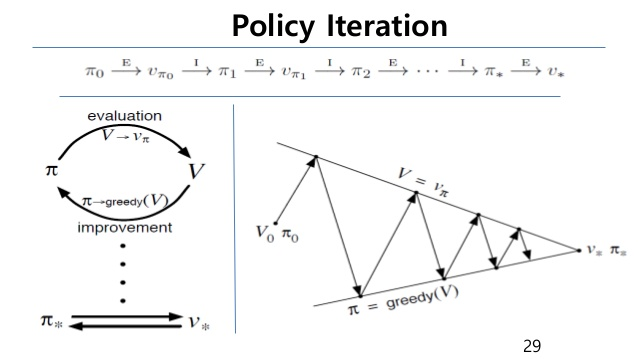
\includegraphics[width=\linewidth]{policy_iteration.jpg}
  \caption{Policy iteration algorithm (~\cite{Sutton:1998:IRL:551283}).}
  \label{fig:policy_iteration}
\end{figure}
The algorithm starts from a random policy, $\pi_0$, as shown in Figure ~\ref{fig:policy_iteration}. The policy iteration phase tried to extract the value function of the current policy. This can be done in various ways, mentioned in the previous section. The closed form solution could be used to get an exact solution(~\ref{eq:mdp_closed_form_solution}), but as we said before this comes with a high computational cost. Alternatively, we can apply recursively the Bellman Expectation Operator, which, as mentioned before, is a contraction in the max norm. By applying recursively this operator we get an approximation of the real value function of the policy, but for most applications look for an approximation of the value function. In fact in \emph{modified policy iteration}~\cite{Puterman:1978:MPI:2828482.2828486} the algorithm does not wait until convergence, advocating that a sufficiently good approximation is enough.\par
After the policy evaluation phase, policy improvement generates the greedy policy from the value function, by selecting, in each state, the action that maximizes it.
\begin{equation}
	\pi^{t+1}(s)=\argmax_{a \in \mathcal{A}} Q^{\pi^t}(s,a) \qquad \qquad s \in \mathcal{S}
\end{equation}
The policy generated is deterministic , and moreover it is guaranteed to be an improvement over the previous one.
\begin{theorem}
(Policy Improvement Theorem) Given an MDP $\mathcal{M}$ and two deterministic policies $\pi$ and $\pi′$ :
\begin{equation*}
	Q^\pi(s,\pi'(s)) \geq V^\pi(s) \qquad \forall s \in \mathcal{S} \qquad \Rightarrow \qquad V^{\pi'}(s) \geq V^\pi(s)	\qquad \forall s \in \mathcal{S}
\end{equation*}
\end{theorem}
Now, of course, by evaluating the policy by means of the value function, to generate the greedy policy, we need the state transition model, $\mathcal{P}$. In other cases, when the model is not available, Q-iteration is used. Here, instead of evaluating the value function of the policy, we evaluate the action-value function in a similar way.
\subsection{ Value Iteration}
Value iteration finds the optimal value function (and from it the optimal policy), without the intermediate use of policies. This method is based on the iterative application of the Bellman Optimality operation discussed in the previous section.\par
We recall that this operator is a contraction ~\cite{Banach1922}. The algorithm start from an initial (random) value function, $V^0$, and applies iteratively the Bellman operator until a stopping condition is met. The stopping condition might be maximal number of iterations or based on some minimal metric of distance between two subsequent estimations of the value function. In the end the optimal policy is recovered in the same way as in policy iteration, by taking the greedy policy induced by the optimal value function. Again the state transition model is required, otherwise we need to estimate the optimal action-value function instead.The convergence to the optimal value function is guaranteed. In particular, given two consecutive
approximations of the optimal value function we can bound the error \wrt the true optimal value function:
\begin{equation}
\|V^{t+1}-V^{s}\|_{\infty} < \epsilon \qquad \Rightarrow \qquad \|V^{t+1}-V^*\|_{\infty} < \frac{2 \epsilon \gamma}{1- \gamma}.
\end{equation} \par
While policy iteration represents explicitly the policy, value iteration focuses on the value function only. This means that intermediate value functions may not correspond to any policy. Both have polynomial time complexity for MDPs with fixed discount factor ~\cite{DBLP:journals/corr/abs-1301-6718}. Considering the single iteration, policy iteration is more computationally demanding \wrt, value iteration since it requires evaluating the policy and performing the greedy improvement, but it tends to converge in a smaller number of iterations. Besides DP, also Linear Programming (LP) can be employed to recover the optimal value function. However, LP becomes impractical at a much smaller number of states than DP methods do.
\section{Reinforcement Learning} \label{reinforcement_learning}
The main disadvantage of Dynamic Programming (when used to solve MDPs) is the fact that it requires the knowledge of the model. We need the state transition model to solve the MDP, which in real life problems is, more often than not, unavailable. Furthermore, DP becomes quickly infeasible as the action-state spaces of the MDP increase and it is clearly inapplicable for infinite MDPs. Reinforcement Learning tries to  convert DP algorithms in a sample-based nature. Sample based because we need to identify the underlying mechanisms of the environment since we do not have the transition model. 
\subsection{Classifying Reinforcement Learning Algorithms}
Reinforcement Learning, being one of the Machine Learning paradigms, is a vast field containing a large number of algorithms. We can classify RL algorithms in a number of ways as:
\begin{itemize}
\item Model-based vs Model-free depending whether or not the algorithm needs the state transition probabilities, $\mathcal{P}$. Model-free techniques try to find the optimal policy directly from samples of trajectories, whereas model-based techniques estimate first the transition model, to then apply DP to find the optimal policy
\item On-Policy vs Off-Policy depending on whether the agent learns the same policy used to collect data. On-policy algorithms learn the value function of the policy used to collect the samples, whereas off-policy algorithms learn the value function of a second policy (typically the optimal policy) while using a different policy to collect the samples.\
\item Online vs Offline depending on when the learning is performed. Online methods learn while collecting the samples whereas offline methods learn after they have all the data.
\item Tabular vs Function Approximation depending on the representation of the value function. Tabular methods explicitly save the value function for each state in a table (usable only in finite MDPs), whereas function approximation algorithms use approximators (regressors, neural networks) to estimate the value function.
\item Value-based vs Policy-based vs Actor Critic. Value-based algorithms estimate the value-function of the optimal policy (and from it the optimal policy). Policy-based algorithms try to estimate directly the optimal policy. Actor-critic methods have two parts. An actor(agent) that estimates the value function and a critic that updates it.
\end{itemize}
\subsection{Model-free Prediction}
The prediction problem aims to estimate the value function of a given policy.We will concentrate on the \emph{model-free} case, \ie when the transition model of the MDP is not known. We recall the process is now an MRP (MDP+ policy). The focus will be on two classes of algorithms, \emph{ Monte Carlo approches} (MC) and \emph{Temporal Difference approaches} (TD) ~\cite{Sutton:1998:IRL:551283}.Both methods are able to learn the value function of the policy directly from episodes of experience, whithout knowing the transition model of the MDP.They are able to do this by iteratively updating their estimation of the value function in each state.The updates are done using the exponential average update rule :
\begin{equation}
	V^{t+1}(s_t)=V^{t}(s_t)+ \alpha^t\left(v^{*}_t-V^{t}(s_t) \right),
\end{equation}
where $v^{*}_t$ is an estimation of the value function in state $s_t$ and $\alpha^t$ is the learning rate.\par
The two approaches differ on how the estimator $v^{*}_t$ is calculated. Monte Carlo learning:
\begin{itemize}
	\item Uses the simplest possible idea , value function is the sum of  (discounted) returns, $v^{MC}_{t}=\sum_{i=t}^{T(\tau)-1} \gamma^{t} r_{i+1}$;
	\item The approximator $v^{*}_t$ has the disadvantage the method is only usable for episodic MDPs. All episodes must terminate for the value function to be estimated;
	\item For the same reason can only be used for offline learning;
	\item States may be visited multiple times during an episode. When this happens we can either compute the value function just for the first visit of the state (first-visit MC) or for every time we visit the state (every-visit MC).The choice between the two boils down to the classical bias-variance trade off.~\cite{Sutton:1998:IRL:551283}.
\end{itemize}\par
TD on the other hand:
\begin{itemize}
	\item Leverages on bootstrapping to use the crrent approximation of the value function;
	\item The estimator is now the \emph{temporal difference target}, given by $v^{TD}_t=r_{t+1}+ \gamma V^{t}(s_{t+1})$;
	\item Bootstrapping allows for online learning and is not restricted to episodic MDPs;
	\item Bootstrapping after multiple timesteps gives rise to the $TD(\lambda)$ class of algorithms. We refer to ~\cite{Sutton:1998:IRL:551283} for more details.
\end{itemize}\par
Even though it can be shown that MC is an unbiased estimator ~\cite{Sutton:1998:IRL:551283} and TD is biased , in practice $TD(\lambda)$ is used more since it exploits the Markovian property of MDPs.
\subsection{Model-free Control}
The prediction problem deals with evaluating the value function a given policy. Whats more interesting about RL algorithms is the ability to learn a optimal policy in an MDP from samples of experience. This is called the \emph{model free control problem}. Control algorithms can be derived from the algorithms mentioned in the previous section by modifying them in a DP fashion. The main modification is estimating the Q function instead of the value function, since the model of the environment is not given. Second, and most importantly, we cannot apply the policy improvement step just by choosing the optimal action according to our current estimate. We are learning from samples, starting from an initial (possibly random) estimate.By choosing the optimal action, completely trusting our current estimate, we (almost surely) will converge to sub-optimal policies, since the samples we collect depend on our estimation of the Q function. This is in fact an instance of the \emph{exploitation vs exploration} problem. Do we use the information we have so far (exploitation) or we chose new actions to gather new informations (exploration) ? \par
An option is using an $\epsilon-greedy$ policy, a stochastic policy that chooses a random action, from the available ones, with probability $\epsilon$ and the current optimal action with probability  $1-\epsilon$. The $\epsilon-greedy$ Policy Improvement Theorem ~\cite{Sutton:1998:IRL:551283} shows that the new policy is an improvement \wrt, the previous one. As we collect samples, we become more confident about our estimate of the Q function and we can explore less. This can be done, in the simplest case, by defining a schedule for the \emph{exploration rate} $epsilon$, so that it converges to zero.We can now write the update rule for the Q function as :
\begin{equation}
	Q^{t+1}(s_t,a_t)=Q^{t}(s_t,a_t)+ \alpha^t\left(v^{*}_t-Q^{t}(s_t,a_t) \right).
\end{equation}
Again, different algorithms differ on their estimation of the value function, $v^{*}_t$.
MC uses the estimator $v^{MC}_{t}=\sum_{i=t}^{T(\tau)-1} \gamma^{t} r_{i+1}$, while TD as before uses $v^{TD}_t=r_{t+1}+ Q^{t}(s_{t+1},a_{t+1})$. The TD control algorithm is called SARSA ~\cite{rummery:cuedtr94}. The remarks made in the previous section about the usage of the two algorithms are valid also in the control setting. It is important to mention that both MC and TD are on-policy methods, meaning that they estimate the value function of a policy , while following it. This is important especially while bootstrapping in TD, since it determines the choice of the next action, $a_{t+1}$ that appears in the TD target. Both algorithms have convergence guarantees, as long as they follow the Robbin-Moore conditions on the learning rate, given by:
\begin{equation}
	\sum_{t=0}^{\infty} \alpha^{t}=+\infty \quad and \quad \sum_{t=0}^{\infty} \left(\alpha^{t}\right)^2 \leq +\infty.
\end{equation}
and  each state-action pair is visited infinitely many times ~\cite{Jaakkola:1994:CSI:1362288.1362296,Sutton:1998:IRL:551283}. A simple case that respects these conditions is $\alpha^t= \frac{1}{t}$.\par
We will now shortly present, an off-policy algorithm, used to estimate the optimal action-value function of an unknown MDP. The famous Q-Learning ~\cite{Watkins:89} can be thought as an extension of Value Iteration to the model-free case. Basically it applies a sample based version of the Bellman Optimality Equation, allowing to learn the optimal action value function without having to actually play an optimal policy The update rule of Q learning is given as:
\begin{equation}
	Q^{t+1}(s_t,a_t)= Q^{t}(s_t,a_t) +\alpha^t \left(r_{t+1} + \gamma \max_{a' \in \mathcal{A}} Q^{t}(s_{t+1},a') - Q^{t}(s_t,a_t)\right).
\end{equation}
Pseudocode of the Q learning algorithm is shown in Alg. [~\ref{alg:q-learning}].
\begin{algorithm}[H]
\begin{flushleft}
        \textbf{Input:} States $\mathcal{S} = \{1, \dots, n_s\}$, Actions $\mathcal{A} = \{1, \dots, n_a\}$, Reward function $R: \mathcal{S} \times \mathcal{A} \rightarrow \mathbb{R}$, Learning rate $\alpha \in [0, 1]$, Exploration rate $\epsilon \in [0, 1]$, Discount factor $\gamma \in [0, 1]$.\\
        \textbf{Input:} $Q$ function
\end{flushleft}
        \begin{algorithmic}
            \State Initialize $Q: \mathcal{S} \times \mathcal{A} \rightarrow \mathbb{R}$ arbitrarily
            \While{$Q$ is not converged}
                \State Start in state $s \in \mathcal{S}$
                \While{$s$ is not terminal}
                    
                    \State Chose $a$ according to Q and  $\epsilon-greedy $ exploration strategy 
                    \State Take $a$ and receive the reward $r$ and the new state $s'$
                    \State $Q(s', a) \gets (1 - \alpha) \cdot Q(s, a) + \alpha \cdot (r + \gamma \cdot \max_{a'} Q(s', a'))$
                    \State $s \gets s'$
                    \State Update learning rate $\alpha$ according to learning rate schedule
                    \State Update exploration rate $\epsilon$ according to exploration rate schedule
                \EndWhile
            \EndWhile
            \Return $Q$
        \end{algorithmic}
    \caption{$Q$-learning: Learn function $Q: \mathcal{S} \times \mathcal{A} \rightarrow \mathbb{R}$}
    \label{alg:q-learning}
\end{algorithm}
\section{Function Approximation} \label{sec:function_approximation}
Q-learning uses a tabular representation for the Q-function which is inapplicable when the state-action space is large, due to memory and time restrictions. Obviously, when the MDP is continuous a tabular representation is impossible. The solution proposed in literature is to estimate the value function with function approximation, i.e., $V^\pi(s) \approx \hat{V}(s)$. This approach tends to enforce generalization capabilities of the model and to speed up the computation \wrt tabular representation with no significant performance degradation when the approximators are carefully chosen.\par 
We can distinguish between parametric and non-parametric approximators: the former have a set of parameters known a priori, data are used to tune the values of the parameters (e.g., \emph{neural networks}); while for the latter the number of parameters is not fixed (e.g., \emph{decision trees}, \emph{nearest neighbors}).
\subsection{Basics of Function Approximation}
In the context of function approximation, learning can be defined as the process of
selecting a function $\hat{V}$ in a functional space $\mathcal{F}$ in order to minimize a loss function that encodes the fact that we aim to use $\hat{V}$ to approximate the value function $V^\pi$. We aim to solve the following problem:
\begin{equation}
\hat{V} = \argmin_{f \in \mathcal{F} } \Vert V^\pi - f \Vert_{q}.
\end{equation}
A fundamental issue at this point, is the \emph{bias-variance trade off}, closely related to the choice of the function space $\mathcal{F}$ ~\cite{hastie01statisticallearning}. We will focus on parametric function approximation, in which $\mathcal{F} = \mathcal{F}_\theta = \{f_\theta : \theta \in \Theta \subseteq \mathbb{R}^k \}$ is a parametric function space. The problem of finding $\hat{V}$, becomes equivalent to finding the optimal parameter:
\begin{equation}
 \hat{\theta} = \argmin_{\theta \in \Theta} \Vert V^\pi - f_{\theta} \Vert_{q}.
 \label{eq:loss_function_func_approximator}
\end{equation}
We assume that function $f_\theta$ is constructed starting from a vector of \emph{features} $\phi = \phi_1 , \phi_2 , \ldots, \phi_p$ , \ie functions that map each state to real numbers $\phi(s)$ (or each state-action pair to real numbers $\phi(s, a)$). The functional form of $f_\theta$ can vary a lot: from linear models to complex non linear approximators, like neural networks.\par
Under certain regularity conditions, prediction in this scenario can be carried out with \emph{gradient descent} methods employing as \emph{loss function} equation (\ref{eq:loss_function_func_approximator}) with $q=2$ and the unknown value function is replaced with the corresponding Monte Carlo or Temporal Difference estimator. The parameter update for approximate prediction is given by:
\begin{equation}
\theta^{(t+1)} \leftarrow \theta^{(t)} - \alpha^{(t)}(v^*_t - f_{\theta^{(t)}}(s_t,a_t)) \nabla_{\theta} f_{\theta^{(t)}}(s_t,a_t).
\end{equation}
Unfortunately convergence is no longer guaranteed. SARSA may display instability while Q-learning does not have anymore guarantees even for simple linear approximators. \par
The algorithms presented so far perform updates as soon as a sample is drawn
(\emph{incremental methods}). This has at least two drawbacks: first, it is computationally inefficient; second, two subsequent samples are strongly correlated. On the contrary, \emph{batch methods} seek to find the best fitting value function once all the data have been collected. The loss function remains the same, but learning is performed over the whole (static) dataset. This allows recovering the optimal parameters even in closed form for some simple approximators, like linear parametrizations.
\section{Distributional Reinforcement Learning} \label{distributional_rl_section}
The common approach to RL is modeling the expected random return the agent gets, or the value function. This approach has shown really good results, like playing the game of Go in super-human levels, but it has some  problems.Consider for a moment the Atari game , Space Invaders. A frame from this game is shown in Figure ~\ref{fig:space_invaders}. In this game the agent control a laser-canon that shoots alien invaders (hence Space Invaders) as they descent the screen. While the agent shoots enemy spaceships he collects points (rewards). The goal of the game is obviously maximizing this reward. The enemy ships also shoot at the laser-canon. If all the laser-canons of the player are destroyed the game ends and the final score is the score collected so far. What is interesting about the game is that if the enemy ships reach the bottom , you lose immediately, no matter how many lives you have left. This is interesting because as the enemies approach the bottom of the screen, the probability that you lose the game increases so in these states the value distribution is quite complex, multi-modal if you will. A simple expected return does not capture this multi modality and actually gives an expectation that will not be reached in practice. Modeling the expected return of the agent actually hides the intrinsic randomness of the environment. In this section we will discuss the importance of value distributions.
\begin{figure}
  
\includegraphics[width=\linewidth]{space_invaders.jpg}
  \caption{A frame form the video game Space Invaders }
  \label{fig:space_invaders}
\end{figure}
\subsection{Value distributions}
One of the major principles of RL states that, if not not otherwise constrained in its behavior, an agent should aim to maximize its expected utility Q, or value~\cite{Sutton:1998:IRL:551283} and as discussed before this is expressed elegantly with the Bellman Operators.\par
Bellemare et al. ~\cite{DBLP:journals/corr/BellemareDM17} argue for the fundamental importance of the value distribution:  the distribution of the random return received by a reinforcement learning  agent. There is a large body of literature on this distribution~\cite{jaquette1973}~\cite{articleSobel} , but for mainly specific purposes, such as implementing risk-aware behavior~\cite{Morimura:2010:NRD:3104322.3104424} or to model parametric uncertainty~\cite{Dearden98bayesianq-learning}. Specifically we are interested on the random return $Z$.\par
\subsection{Distribution Distance Measures}
In this section we will review some  measures of distance between distributions which will be used in this thesis.
\subsubsection{KL Divergence}
In \emph{mathematical statistics}, the Kullback–Leibler divergence (also called relative entropy) is a measure of how one probability distribution is different from a second, reference probability distribution ~\cite{Kullback59}. In the simple case, a Kullback–Leibler divergence of 0 indicates that we can expect similar, if not the same, behavior of two different distributions, while a Kullback–Leibler divergence larger than 0 indicates that the two distributions behave differently and its value indicates ``how much'' the distributions differ. In simplified terms, it is a measure of surprise. 
\par More formally, given two probability measures, $P$ and $Q$, the KL divergence of $Q$ to $P$, $d_{KL}(P,Q)$ is defined as:
\begin{equation}
d_{KL}(P,Q)=\mathbb{E}_{P}\left[\log\frac{P(z)}{Q(z)}\right].
\end{equation}
$d_{KL}(P,Q)$ is an index of the information gained when one revises one's beliefs from the prior probability distribution $Q$ to the posterior probability distribution $P$. In other words, it is the amount of information lost when $Q$ is used to approximate $P$ ~\cite{BurnhamModelSelection}. In applications, $P$ typically represents the ``true'' distribution of data, observations, or a precisely calculated theoretical distribution, while $Q$ typically represents a theory, model, description, or approximation of $P$. In order to find a distribution $Q$ that is closest to $P$, we can minimize KL divergence and compute an information projection.
\subsubsection{Wasserstein Metric}
The Wasserstein metric, $d_p$ is a \emph{distance function} defined between cumulative distributions functions ~\cite{bootstrapAsymptotic}. Given $F$ and $G$, two \emph{c.d.fs}, the Wasserstein metric is defined as:
\begin{equation}
	d_p(F,G)= \inf_{U,V}\Vert U-V\Vert_p,
\end{equation}  
where the infimum is taken over all pairs of random variables $(U,V)$, with respective cumulative distributions $F$ and $G$. For $p< \infty$, and if $U$ and $V$ are defined over $\mathbb{R}$, $d_p$ can be written as:
\begin{equation}
	d_p(F,G)=\left(\int_{0}^{1} |F^{-1}(u)-G^{-1}(u)|^p du \right)^{\frac{1}{p}}.
\end{equation}
Given two random variables $U,V$ with c.d.fs $F_U,F_V$, we will write $d_p(U,V)=d_p(F_U,F_V)$ for convenience.\par
Considering a scalar $a$ and a random variable $A$, independent of $U,V$, the metric $d_p$ has the following properties ~\cite{DBLP:journals/corr/BellemareDM17}:
\begin{equation*}
\begin{split}
		d_p(aU,aV) & \leq \vert a \vert d_p{U,V}, \\
		d_p(A+U,A+V) &  \leq d_p(U,V) \\,
		d_p(AU,AV) & \leq \Vert A \Vert d_p(U,V).
\end{split}
\end{equation*}
Let $\mathcal{Z}$ denote the space of value distributions. For two value distributions $Z_1, Z_2 \in \mathcal{Z}$ a maximal form of the Wasserstein metric can be defined as: 
\begin{equation}
	\overline{d}_p(Z_1,Z_2)= \sup_{s,a} d_p(Z_1(s,a),Z_2(s,a)).
\end{equation}
\subsection{Policy Evaluation Setting}
We recall that agent following a policy $\pi$ in an uncertain world will experience return $Z^\pi$, defined as the sum of discounted rewards following the trajectory induced by policy $\pi$. The value function $Q^\pi$  describes the expected return  from taking  action $a$  in state $s$, then acting according to $\pi$.
\begin{equation*}
	Q^\pi(s,a)=\mathbb{E}\left[Z^\pi(s,a)\right]=\mathbb{E}\left[\sum_{t=0}^{\infty} \gamma^{t}R(s_t,a_t) \right].
\end{equation*}
We emphasize that $Z^\pi$ describes the intrinsic randomness of the agent's interactions with its environment, rather than some measure of uncertainty about the environment itself~\cite{DBLP:journals/corr/BellemareDM17}. We discussed before how this expectation can be expressed elegantly using Bellman's expectation equation. Now we will take away the expectations in Bellman's equation and use the distribution $Z^\pi$\par
The randomness in the return of the next state can also be expressed in the transition operator $P^\pi: \mathcal{Z \rightarrow Z}$, defined as:
\begin{equation}
\begin{aligned}
	P^\pi Z(s,a) \,{\buildrel D \over =}\ Z(S',A') \\
	S' \sim P(\cdot |s,a) \quad A' \sim \pi(S'),
\end{aligned}
\end{equation} 
where $\,{\buildrel D \over =}\ $ is an equality in distribution. We use the capital letters $S'$ and $A'$ to emphasize the random nature of the next state-action pair. Now we can give the definition of the distributional Bellman operator, $\mathcal{T}^\pi Z \rightarrow Z$, as 
\begin{equation}
	\mathcal{T}^\pi Z(s,a) \,{\buildrel D \over =}\ R(s,a)+ \gamma P^\pi Z(s,a).
	\label{eq:bellman_distributional}
\end{equation} 
The \emph{distributional Bellman operator} states that the distribution of $Z$ is characterized by the interaction of three random variables: 
\begin{itemize}
	\item the reward $R$;
	\item the next state-action ($S',A'$);
	\item the random return in the next state-action. $Z(S',A')$
\end{itemize}
Further it can be shown that equation ~\ref{eq:bellman_distributional} is a contraction mapping in Wasserstein metric and its unique fixed point is $Z^\pi$~\cite{DBLP:journals/corr/BellemareDM17} 
\begin{equation}
	\overline{d}_p(T^{\pi}Z_1,T^{\pi}Z_2) \leq \gamma \overline{d}_p(Z_1,Z_2).
\end{equation}
In  this  context,  the  Wasserstein metric is particularly interesting because it does not suffer from disjoint-support issues ~\cite{pmlr-v70-arjovsky17a} which  arise  when  performing  Bellman  updates.
\subsection{The Control Setting}
In the previous section we discussed how the Bellman distributional operator has the same properties as the expectation one. This does not hold in the control setting unfortunately, with the optimality operator. As a reminder, in the control setting we seek a policy $\pi$ that maximizes the value function and the corresponding notion of an optimal value distribution. We will see how optimality is a trickier concept when seen in a distributional setting.Just like with the value function, the notion of optimal value distribution is tied with the notion of an optimal policy. But if with value functions , all optimal policies have the same optimal value function , this is not the case with value distributions. \par
The notion of optimal policy does not change. The optimal policy is still the policy that maximizes the expected return. Having the definition of the optimal policy , we can define the optimal value distribution as :
\begin{definition}
	An optimal value distribution is the value distribution of an optimal policy. The set of optimal value distributions is  $\mathcal{Z^*} := \left\lbrace \mathcal{Z^{\pi^*}} : \pi^* \in \Pi^* \right\rbrace$
\end{definition}
We emphasize that not all value distributions with expectation $Q^\pi$ are optimal. They must match the full distribution  of the return under some optimal policy.\par
Recall that the expected Bellman optimality operator $\mathcal{T}$. In (~\ref{eq:bellman_optimality}) the maximum over actions corresponds to an implicit greedy policy, which cannot be ignored in the distributional case. So let us give the definition of a greedy policy as provided by ~\cite{DBLP:journals/corr/BellemareDM17}.
\begin{definition}
	A greedy policy $\pi$ for $Z \in \mathcal{Z}$ maximizes the expectation of $Z$. The set of greedy policies for $Z$ is:
	\begin{equation*}
	\mathcal{G}_{Z} = \left\lbrace \pi : \sum_{a \in \mathcal{A}} \pi(a|s) \mathbb{E}\left[Z(s,a)\right] =\max_{a' \in \mathcal{A}} \mathbb{E} \left[Z(s,a')\right] \right\rbrace.
	\end{equation*}
\end{definition}
After defining the notion of a greedy policy we can define a distributional optimality operator as any operator $\mathcal{T}$ which implements a greedy selection rule, \ie
\begin{equation}
	\mathcal{T}Z=\mathcal{T}^\pi Z \quad for \quad some \quad \pi \in \mathcal{G}_{Z}.
\end{equation}
 As in the policy evaluation setting, we are interested in the behavior of the iterates $Z_{k+1}= \mathcal{T}Z_k$ where $Z_0 \in \mathcal{Z}$. Bellemare ~\cite{DBLP:journals/corr/BellemareDM17} shows that the expectation, $\mathbb{E}Z$ behaves as expected, converging to $Q^*$ exponentially quickly. Unfortunately, convergence of $Z_k$ to $Z^*$ is neither quick nor assured to reach a fixed point. In Bellemare derives 3 negatives results concerning the operator $\mathcal{T}$:
 \begin{itemize}
 	\item The operator $\mathcal{T}$ is not a contraction in any measure;
 	\item Not all optimality operator have a fixed point $Z^*$;
 	\item Even if $\mathcal{T}$ has a fixed point, it does not guarantee the convergence of $\lbrace Z_k\rbrace$ to $\mathcal{Z^*}$.
 \end{itemize}